\documentclass[11pt,a4paper]{article}

\usepackage{Rapport_Type} %% cibler doc/modules/

\usepackage{fancyhdr}
\fancypagestyle{basdepage}{
\fancyfoot{} % clear all footer fields
\fancyfoot[C]{Stage Lip6 : Amélioration de la réactivité des réseaux p2p pour les MMOGs [\thepage]}
\renewcommand{\headrulewidth}{0pt}
\renewcommand{\footrulewidth}{0pt}}
\pagestyle{basdepage}

\begin{document}
  \fairetitre{Amélioration de la réactivité des réseaux pair à pair pour les MMOGs}{Rapport Type}{Xavier Joudiou}{09/04/10}

\newpage
\tableofcontents

\newpage

\section{Abstract}

	Depuis plusieurs années, une nouvelle classe d'application est apparue. Il s'agit des applications pair à pair, ces applications sont devenues populaires grâce à des applications de partage de fichier. De nombreuses autres utilisations de l'architecture pair à pair existent, comme pour la communication, la distribution de calculs scientifiques, les jeux vidéos multijoueur en ligne, etc. Nous allons nous intéresser aux jeux vidéos massivement multijoueur ( MMOG pour Massively Multiplayer Online Games) qui sont de plus en plus populaires et qui font ressortir des problèmes que l'architecture pair à pair doit pouvoir corriger. Le problème du passage à l'échelle sera l'un des plus importants à résoudre car des milliers de joueurs doivent pouvoir participer en même temps et avec un latence faible.\\ 
	L'architecture pair à pair est la plus adaptée pour résoudre le problème de passage à l'échelle dans les MMOGs, mais il sera plus difficile d'assurer une faible latence. Le but de ce stage est de proposer une technique efficace de prédiction du comportement des joueurs de MMOG afin de pouvoir anticiper leurs mouvements. Il est alors possible d’adapter le réseau en conséquence et ainsi diminuer la latence due au routage.\\ 
	A l'heure actuelle, les MMOGs utilisent une architecture client/serveur, ce qui pose des problèmes de passage à  l'échelle, car on aura un nombre de joueurs limités pouvant être sur chaque serveur. Ce qui fait que le jeu est découpé en plusieurs parties indépendantes, chacune étant gérée par un serveur, ce qui pose des problèmes d'unité de l'univers. Ce problème implique aussi un coût achat de serveur et en maintenance de ceux-ci très élevé.\\
	Pour remédier à cela, une solution consiste à remplacer le modèle client/serveur par un réseau logique pair à pair (overlay).Malheureusement, les protocoles pair à pair existants sont trop peu réactifs pour assurer la faible latence nécessaire à ce genre d’applications. En effet, pour une expérience de jeu satisfaisante, l’information entre deux pairs en interaction dans le MMOG doit être transmise avec une latence d’au plus quelques centaines de millisecondes. Ceci est problématique, même avec un routage efficace.\\
	Néanmoins, quelques travaux ont déjà été menés pour adresser ce problème. L’idée est d’adapter le voisinage de chaque pair afin que toute l’information dont il aura besoin dans un avenir proche se trouve à un seul hop de lui dans le réseau. Il est alors nécessaire de correctement évaluer les futurs besoins de chaque pair, et de faire évoluer son voisinage à temps.
		Le travail à réaliser est d'améliorer un overlay pair à pair pour MMOG qui a été implémenté dans le simulateur Peersim. Cet overlay anticipe les mouvements du joueur dans le MMOG et adapte le voisinage de son pair en conséquence. Cependant, les algorithmes d’anticipation sont naïfs et peu précis .
Il s’agit donc de concevoir des mécanismes efficaces d’anticipation de la trajectoire des joueurs afin de mieux adapter l’overlay à leurs déplacements et diminuer la latence.\\

\textbf{Mots Clés:} Pair à pair, Massively Multiplayer Online Games, Overlay, Anticipation des movements, Collaboration des nœuds ...


\newpage

\section{Introduction}
	Le début de ce rapport va permettre d'observer les différents travaux déjà réalisés sur les applications pair à pair. Les jeux vidéos massivement multijoueur étant le principal type d'application qui va nous intéresser. Ces applications, regroupant un grand nombre de personnes, impliquent que différentes propriétés (jouabilité, fluidité, réactivité, etc) soient vérifiées. L'architecture pair à pair peut répondre efficacement à certaines des différentes propriétés nécessaires au bon fonctionnement des applications mais un problème peut se poser au niveau de la latence. Le but du stage a été d'améliorer le voisinage logique du réseau pair à pair pour que l'utilisateur puisse avoir dans son voisinage les données. Ces données lui seront nécessaires aux instants suivantes dans l'environnement, pour cela il faut anticiper au mieux les mouvements du joueur.\\

	Tout d'abord nous expliquerons pourquoi l'approche pair à pair est celle qui paraît la plus adaptée pour répondre aux différentes problématiques qu'induisent ces applications, nous en profiterons pour rappeler rapidement les caractéristiques des différentes architectures (cf \ref{whyp2p}, page \pageref{whyp2p}). Ensuite, les mécanismes permettant une meilleure mise en place de l'architecture pair à pair seront expliqués, nous rentrerons un peu plus dans les détails pour Solipsis (cf \ref{solipsis}, page \pageref{solipsis}). Solipsis est un travail qui propose un monde virtuel entièrement décentralisé et scalable. Un overlay qui est caractérisé par une forte malléabilité applicative, sert de support au monde virtuel. Après avoir parlé des différents mécanismes existants qui ne prennent pas en compte la mobilité, une étude des traces des avatars dans les environnements virtuels sera alors introduite (cf \ref{trace}, page \pageref{trace}). Cette étude des traces permettra de mieux expliquer les différentes solutions d'amélioration de la réactivité du réseau pair à pair. Ensuite, le travail Blue Banana qui a permis de mettre en place une première amélioration, au fonctionnement du monde virtuel proposé par Solipsis, sera expliqué (cf \ref{BlueBanana}, page \pageref{BlueBanana}). Blue Banana permet d'anticiper les mouvements des avatars, pour ainsi adapter au mieux le voisinage des nœuds. \\

	
	Ensuite, les deux principales améliorations, qui ont été mises en place durant ce stage, seront présentées. La première solution consiste à intégrer un cache dans les nœuds du réseau, son fonctionnement et ses performances seront expliqués. L'autre solution, implémentés durant le stage, est une amélioration du préchargement des données qui a été mis en place dans Blue Banana. Outre l'explication des résultats de chacune des solutions, les différentes implémentations explorées seront présentées. Enfin les autres pistes d'amélioration, qui ont été envisagées, seront expliquées.



\newpage
\section{Premier point}
	\subsection{Petit A}
	Petit A \\
	\subsection{Petit B}
	Petit B \\
	
\newpage
\section{Deuxieme point}
	\subsection{Petit A}
        Petit A \\
	Comme il est très bien dit dans \cite{1613041}\\
	\par suite Petit A
	\newpage
	\subsection{Petit B}
        Petit B \\
\newpage
\section{Pourquoi passer à des solutions pair à pair?}
	\label{whyp2p}
	Nous allons voir pourquoi est-il nécessaire de passer d'une architecture Client/Serveur à une architecture pair à pair, nous verrons les différences des deux solutions.
	\subsection{Les solutions existantes}
	Dans la plupart des Massively Multiplayer Online Games, l'architecture est de type client/serveur (voir page ~\pageref{P2P/ClServ}). Dans cette architecture, il a forte distinction entre le client, qui envoie des requêtes au serveur et attend les réponses, et le serveur qui est à l'écoute de requêtes des clients. Cela va simplifier la sécurité et le fonctionnent global des jeux. Par exemple, pour effectuer des updates sur l'état global du jeu, il suffit de le faire sur un seule machine et il n'y aura pas de problème d'incohérence entre les données. De même pour la sécurité, toutes les données étant regroupées sur une seule machine, le contrôle sera beaucoup plus simple que dans des systèmes distribués où le nombre de point d'entrée sera beaucoup plus important. \\
	Le problème est que cette architecture ne passent pas à l'échelle, le serveur devient un goulot d'étranglement et si un trop grand nombre de joueurs se connecte, le serveur ne tiendra pas. Le problème est résolu "temporairement?" en ayant des serveurs de très grandes capacités ou en mettant en place des clusters de serveur \textbf{(voir bibli)}. Mais ces solutions induisent un gros investissement dès le début de la mise en service du jeu et elles sont très chères en coût de maintenance. Un autre problème est le disponibilité du système en cas de panne du serveur, si le serveur tombe en panne alors plus personne n'aura accès à l'application que ce dernier faisait fonctionner. \\
	Au vue du nombre croissant de participant à ce genre de jeux vidéos massivement multi joueur, le passage à l'échelle devient un sujet très important et c'est pour cela que les recherches sur des architectures distribuées sont de plus en plus importantes textbf{(voir si statistiques)}. \\
\newline


	\subsection{Les avantages et les inconvénients du pair à pair}
	Comme il est dit avant, l'augmentation croissante des recherches sur le sujet atteste du fait que des problématiques ressortent des solutions existantes. Le problème du passage à l'échelle est sûrement le plus important et est l'une des raisons de ces recherches. Les architectures pair à pair ne font plus ressortir d'entité serveur et client, chaque nœud sera client et serveur en fonction du moment (voir page ~\pageref{P2P/ClServ}). Les systèmes pair à pair peuvent avoir une multitude d'utilisation, que ce soit dans le partage de fichier, la communication, les jeux vidéos , le calcul scientifique, le militaire, etc. \\
	L'architecture pair à pair est faite telle qu'il n'y a pas de goulot d'étranglement, nous passons d'un système où tout passait par un point unique à un système qui comporte un grand nombre d'entité qui peuvent toutes avoir le même rôle. L'utilisation de cette architecture peut entrainer un grand nombre de communications, elle nécessite des synchronisations des entités, des gestions des ressources partagées et d'autres problèmes ( \textbf{A REVOIR}), il faut donc trouver des solutions à tous ces problèmes éventuels. Elle est donc plus adapté à des applications massivement multi joueur mais il faut pouvoir garantir les mêmes propriétés que les systèmes client/serveur. A REVOIR\\
	Les systèmes pair à pair sont par exemple plus difficile à surveiller, les phénomènes de tricherie sont plus difficiles à surveiller, de même pour tout ce qui est sécurité. Nous avons pu voir qu'il existe trois type de tricherie: par Confidentialité, c'est à dire d'obtenir des informations non autorisées sur d'autres utilisateurs; par Intégrité, si il y des modification du monde, des lois physiques ou les lois du jeu non autorisées; par Availability, c'est le fait de provoquer des ralentissements ou des arrêts de parie du jeu ( référence vers Challenges in P2P gaming). Il faut que le système soit aussi fiable sur le long terme et qu'il soit tolérant aux connexions et déconnexions.

\\ \newline
	
	AJOUTER. Les jeux vidéos ont des avantages qui font qu'il sera plus aisé de réaliser une distribution~\cite{1267692}:
	\begin{itemize}
		\renewcommand{\labelitemi}{$\bullet$}
		\item Les jeux vidéos tolèrent une consistence faible pour les différents états de l'application.
		\item Il est assez aisé de prédire les écritures et les lectures grâce à l'ensemble des règles définies dans le jeu. 
	\end{itemize}
	\vspace{1.5cm}
	\begin{figure}[!h]
	\centering
	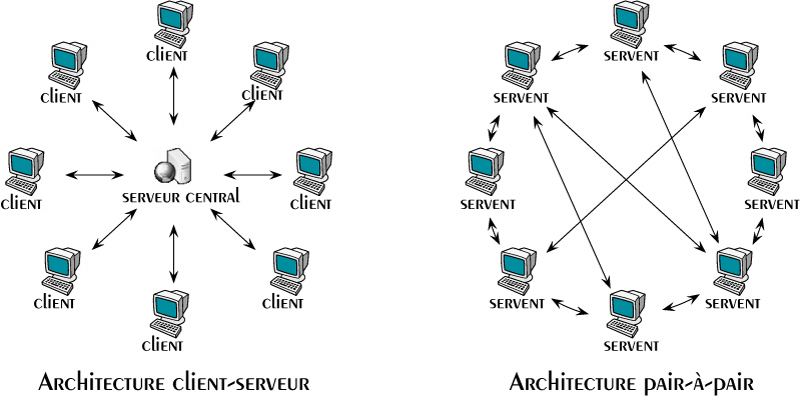
\includegraphics[width=15cm,height=8cm]{../Images/p2p-85145.png}\\
	\caption{Schéma des architectures pair à pair et client/serveur}
	\label{P2P/ClServ}
	\end{figure}

\newpage
Dans plusieurs articles, on peut retrouver la notion de textit{Area Of Interest} textbf{ajouter citations}. Le principe est de "réduire" la vision des avatars à un cercle autour de lui.

\newpage
\section{Prise en compte de la mobilité: Blue Banana}
	\label{BlueBanana}
	Il nous a été possible de voir, dans les chapitres précédents, des mécanismes qui permettent de faire évoluer le système en réaction à des événements. Solipsis ne pourrait difficilement fonctionner dans un monde avec des traces réalistes. En prenant en compte les études des traces des joueurs, Blue Banana a permis de mettre en place un mécanisme d'anticipation des mouvements des avatars pour mieux s'adapter.
	\par Blue Banana présente une solution aux différents problèmes que peut rencontrer une architecture pair à pair dans les MMOGs. La mobilité des avatars implique de nombreux échanges de données à travers le réseau pair à pair. Comme les overlays de l'état de l'art n'anticipent pas cette mobilité, les données nécessaires ne seront pas chargées à temps, ce qui conduit à des défaillances transitoires au niveau applicatif. Blue Banana a été réalisée pour résoudre ce problème, il modélise et prédit les mouvements des avatars ce qui permet à l'overlay de s'adapter par anticipation aux besoins du jeux.
	\subsection{Solutions introduites}
	Blue Banana est implémenté au dessus de Solipsis qu'il a été possible d'étudier dans le chapitre~\ref{solipsis}. Plusieurs observations ont été faites et différentes optimisations en sont ressorties. Il nous a été possible d'observer plusieurs types de zone (dense ou non, cf.~\ref{trace}) et que les mécanismes d'adaptation sont trop tardifs pour être mis en place dans la réalité (le chargement des données sera trop lent).
	\subsubsection{Les états de l'avatar}
	\label{Automate}
	Une des premières innovations qui a été introduite est la distinction de plusieurs états d'un avatar. Comme il a été possible de voir dans le chapitre sur la collecte de traces, un avatar se comporte différemment en fonction des zones du monde. Trois états ont donc été introduits:
	\begin{itemize}
	\renewcommand{\labelitemi}{$\bullet$}
		\item \textbf{H}(alted): l'avatar est immobile.
		\item \textbf{T}(ravelling): l'avatar se déplace rapidement sur la carte et il a une trajectoire droite.  
		\item \textbf{E}(xploring): l'avatar est en train d'explorer une zone, sa trajectoire est confuse et sa vitesse est lente.
	\end{itemize} 
	Le changement d'état de l'avatar se fait en fonction de la vitesse de celui-ci, si la vitesse devient supérieure à une borne définie et que l'avatar est dans l'état E alors l'avatar passe en état T. Ce modèle pourrait être affiné par la suite en prenant en compte l'accélération ou l'historique des mouvements. Sur la figure~\ref{automateMob}, nous pouvons mieux distinguer les différents changements d'état. Chaque nœud va agir en fonction de cette automate, il sera initialisé à l'état \textbf{H}(alted). \\
	

	\begin{figure}[!h]
        \centering
        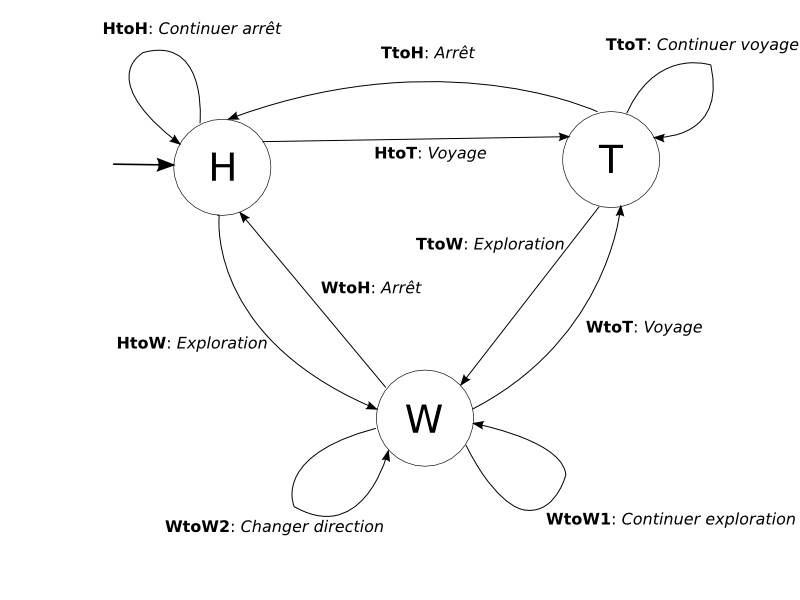
\includegraphics[scale=0.4]{./Ressources/Images/automate.png}
        \caption{\textit{\small Automate décrivant les mouvements d'un avatar. \textbf{En gras}: le nom de la transition, en \textit{italique} sa sémantique}}
        \label{automateMob}
        \end{figure}




	\subsubsection{Anticipation des mouvements}
	Un autre mécanisme a été mis en place, il s'agit d'anticiper les mouvements d'un avatar, pour cela deux suppositions sont faites: seulement une prédiction courte est cohérente, et plus l'avatar se déplace rapidement, plus il y a de chance qu'il continue dans la même direction~\cite{191}. Comme nous pouvons voir sur la figure~\ref{Propa_Algo}, en fonction du vecteur de mouvement de l'avatar, le nœud B, s'il est dans l'état \textbf{T}, va chercher des nœuds qui se trouvent sur la trajectoire probable de l'avatar, tant que son ensemble de voisins n'est pas plein. Le nœud B va envoyer un message aux voisins qui sont le plus près de lui par rapport au vecteur de mouvement. Un mécanisme pour évaluer si le nœud n'est pas trop près, et donc rapatrier des données ne servirait pas car le temps des communications serait supérieur au temps du déplacement de l'avatar. Un des risques est de rapatrier des nœuds qui seront inutiles si l'avatar va changer de direction ou d'état. L'amélioration de ce point fait parti des futures pistes pour améliorer l'algorithme d'anticipation des mouvements.\\
	\vspace{5mm}
        \begin{figure}[!h]
        \centering
        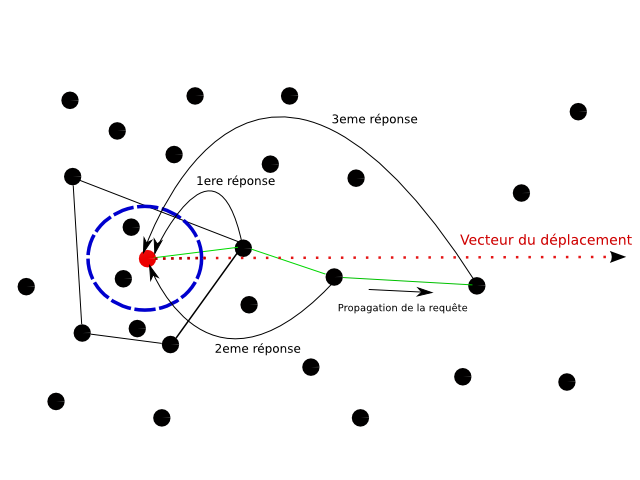
\includegraphics[scale=0.5]{./Ressources/Images/propagation_algo.png}\\
        \caption{Algorithme de propagation}
        \label{Propa_Algo}
        \end{figure}
        \vspace{5mm}
	\subsection{Expérimentations et Résultats}
		Le travail a été testé sur le simulateur à évènements discrets PeerSim ~\cite{peersim}, les expérimentations ont eu pour objectif de comparer Solipsis avec et sans Blue Banana.
		\subsubsection{Le simulateur PeerSim et la description des expérimentations}
		\par PeerSim est un simulateur de réseau pair à pair, qui a deux modes de fonctionnement: par cycles ou par évènements. C'est une API riche et modulaire qui est codée en Java, c'est une composante du projet BISON de l'université de Bologne (Italie). Ce simulateur permet de simuler un large nombre de machines et de tester différentes configurations du réseau. Le simulateur va faire des simplifications sur les couches réseau et les contraintes physiques (latence, pannes, ...). Chaque nœud est considéré comme un module qui va échanger des messages avec les autres nœuds du système. La plupart des plateformes de simulation est basée sur le modèle à évènements discrets. Il est possible de distinguer deux entités: les nœuds et les messages. Le temps va seulement évoluer à chaque nouvel évènement sur un nœud.
		%\subsubsection{Description des expérimentations}
		\par Au départ de la simulation, une carte initiale des traces est introduite dans le simulateur, la carte provient d'une étude de La et Michiardi~\cite{LM-wosn08} dans Second Life. Ensuite, le simulateur va initialiser l'overlay de Solipsis et vérifier que les deux règles de Solipsis sont bien respectées sur chaque nœud, nous insérerons ensuite le reste des traces. Il faut aussi régler les différents paramètres du simulateur (nombre d'avatar, surface du monde, densité, accélération des avatars, vitesse de connection, etc). Plusieurs métriques sont mises en place pour évaluer les résultats:
	\begin{itemize}
	\renewcommand{\labelitemi}{$\bullet$}
		\item \textit{Violation of Solipsis fundamental rules}: Regarde si les propriétés de \textit{Global Connectivity} et de \textit{Local Awareness} sont respectées.
		\item \textit{Knowledge of nodes ahead of the movement}: Mesure pour les avatars qui se déplacent rapidement, le temps moyen pour qu'il connaisse un nœud qui sera sur sa trajectoire.
		\item \textit{Exchanged messages count}: Mesure l'impact de Blue Banana sur le réseau, cela va compter le nombre de messages introduits par Blue Banana et Solipsis.
	\end{itemize}
		\subsubsection{Les résultats}
		Les résultats les plus intéressants montrent que Blue Banana diminue les transitions en échec de 55\% à 20\%, augmentent la connaissance des prochains nœuds de 270\% et cela en créant un overhead de seulement 2\%. Les résultats montrent que le mécanisme d'anticipation introduit par Blue Banana aide l'overlay de Solipsis à s'adapter à temps et à réduire significativement le nombre de violation des règles de Solipsis (de 55\% ou 80\% à 20\%). 

\newpage
\bibliographystyle{plain}
\bibliography{Biblio}


 

\end{document}

